\chapter{Derivation and training of the probabilistic model for cell type classification } \label{app:model_deriv}

\section{Model derivation }

To compute the cell type assignment probability for a given cell type $i$ using the model proposed in Section~\ref{sec:sc_new_model}, we compute
$$p(y_i=1 \mid \bold{x}) = \sum_{k=1}^K \int_{\bold{z}} p\left(y=1 \mid \bold{z}\right) p\left(\bold{z} \mid \bold{x}, k\right) p\left(k \mid \bold{x}\right) \ d\bold{z}$$
We will then derive closed-form equations for each term in the integral.

First, $p\left(y=1 \mid \bold{z}\right)$ is provided by the trained logistic regression classifiers. Specifically,
$$p\left(y=1 \mid \bold{z}\right) := \sigma\left(\boldsymbol{\beta}_i^T\log(\bold{z}+1)\right) $$
where $\boldsymbol{\beta}_i$ are the coefficients in the logistic regression model trained to classify cell type $i$ (the log is take over $\bold{z}+1$ since these models were trained on log(CPM+1) features). 

Next, we derive $p(\bold{z} \mid \bold{x}, k)$:
\begin{align*}
p(\bold{z} \mid \bold{x}, k) &\propto p(\bold{x} \mid \bold{z}, k)p(\bold{z} \mid k)\\
&= \prod_{i=1}^G f_{\text{Poisson}}(x_i ; z_is)f_{\text{Gamma}}(z_i ; a_{k,i}, b_{k,i})\\
&= \prod_{i=1}^G \left[\frac{(z_is)^{x_i} \exp(-z_is)}{x_i!}\right]\left[z_i^{a_{k,i}-1}\exp(-b_{k,i}z_i)\right] \\
&\propto \prod_{i=1}^G \underbrace{z_i^{x_i + a_{k,i} - 1}\exp(-z_i(s + b_{k,i}))}_{\text{kernel of the gamma density function}}
\end{align*}
Therefore,
$$p(\bold{z} \mid \bold{x}, k) = \prod_{i=1}^G f_{\text{Gamma}}(z_i ; x_i + a_{k,i}, s + b_{k,i})$$


Next, we derive $p(k \mid \bold{x})$, the probability that mixture component $k$ generated $\bold{x}$:
$$p(k \mid \bold{x}) \propto \phi_k \int_{\bold{z}}  \prod_{i=1}^G f_{\text{Poisson}}(x_i ; z_is)f_{\text{Gamma}}(z_g ; a_{k,i}, b_{k,i}) d\bold{z}$$
Let $b_{k,i} := \frac{1-p_i}{p_i}$.  Then,
\begin{align*}
p(\bold{x} \mid k) &\propto \phi_k \int_{\bold{z}} \prod_{i=1}^G \left[ \frac{ (z_is)^{x_i} \exp(-z_is) }{ x_i!} \right] \left[ \frac{   z_i^{a_{k,i} - 1} \exp\left(-z_i \frac{1-p_i}{p_i} \right)   }{  \left(\frac{p_i}{1-p_i}\right)^{a_{k,i}} \Gamma(a_{k,i})      } \right] d\bold{z} \\ 
&= \phi_k \prod_{i=1}^G \left[\frac{s^{x_i}(1-p_i)^{a_{k,i}} p_i^{-a_{k,i}} }{x_i!\Gamma(a_{k,i})}\right]  \int_{\bold{z}} \prod_{i=1}^G  \underbrace{z_i^{x_i + a_{k,i} -1} \exp\left[-z_i\left(s + \frac{1-p_i}{p_i}\right) \right]}_{\text{Unnormalized density function of Gamma distribution}} d\bold{z} \\
&= \phi_k \prod_{i=1}^G \left[ \frac{s^{x_i}(1-p_i)^{a_{k,i}} p_i^{-a_{k,i}} }{x_i!\Gamma(a_{k,i})}\right]   \underbrace{\left[ \frac{\Gamma(x_i + a_{k,i})}{\left(s + \frac{1-p_i}{p_i}\right)^{x_i+a_{k,i}}}\right]}_{\text{Inverse normalizing constant}} \\
&= \phi_k \prod_{i=1}^G \frac{\Gamma(x_i + a_{k,i}) }{x_i!\Gamma(a_{k,i})} \left(\frac{sp_i}{sp_i+1-p_i}\right)^{x_i} \left(1 - \frac{sp_i}{sp_i + 1 - p_i}\right)^{a_{k,i}} \\
&= \phi_k \prod_{i=1}^G \frac{\Gamma(x_i + a_{k,i}) }{x_i!\Gamma(a_{k,i})} \left(\frac{s}{s+b_{k,i}}\right)^{x_i} \left(1 - \frac{s}{s + b_{k,i}}\right)^{a_{k,i}} \\
&= \phi_k \prod_{i=1}^G f_{\text{NegBin}}\left(x_i ; a_{k,i}, \frac{s}{s + b_{k,i}}\right)
\end{align*}
Thus,
$$p(\bold{x} \mid k) = \frac{\phi_k \prod_{i=1}^G f_{\text{NegBin}}\left(x_i ; a_{k,i}, \frac{s}{s + b_{k,i}}\right)}{\sum_{k'=1}^K \phi_k' \prod_{i=1}^G f_{\text{NegBin}}\left(x_i ; a_{k',i}, \frac{s}{s + b_{k',i}}\right)}$$

 Finally, 
$$p(k) := \phi_k$$is a parameter of the model.  

Putting all of this together, we arrive at
$$p(y_i=1 \mid \bold{x}) = \sum_{k=1}^K \phi_k p(k \mid \bold{x}) E_{\bold{z} \sim \text{Gamma}(\bold{x} + \bold{a}_k, s + \bold{b}_k)} \left[\sigma\left(\boldsymbol{\beta}_i^T\log(\bold{z}+1)\right) \right]$$


\section{Estimation of gamma distribution parameters }

We explored two approaches for estimating the parameters of the gamma distribution from a set of samples in a given cluster. In the first approach, we simply use the method of moments. However, because some clusters consisted of very few samples (in some cases, only two samples), the estimate of the variance was not robust. We therefore tested an empirical Bayes-like approach to smooth the variances across these clusters. Specifically, for each gene in each cluster, we compute the mean expression of that gene in units of log-CPM as well as the log of the coefficient of variation (CV) (i.e. the ratio of the standard deviation of the CPM to the mean CPM). We then fit a univariate spline to the entire set of expression, CV pairs across all clusters (Fig.~\ref{fig:mean_vs_cv}). We then use this spline to map each mean expression to a variance that is to be used for the calculation of the gamma distribution's shape and rate parameters.  We found that this approach to estimating the gamma distribution parameters produced a slight improvement in classification accuracy over the standard method of moments (Fig.~\ref{fig:shrinkage}).

\begin{figure}[htbp]
    \centerline{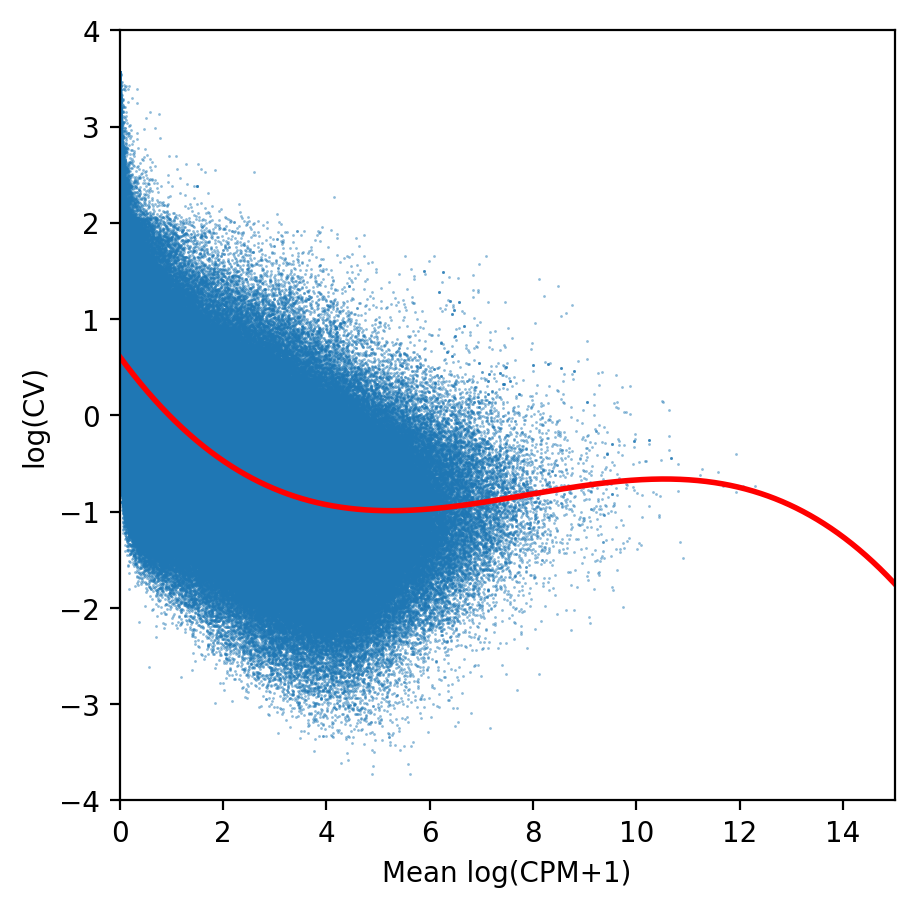
\includegraphics[width=9cm]{figures/mean_vs_coef_of_var.png}}
    \caption{\textbf{Fitting mean expression to coefficient of variation.} A scatterplot comparing mean log(CPM+1) expression values to the log of the coefficient of variation for the CPM expression values. We fit a univariate spline (red) to this data for use in the empirical Bayes-like estimation procedure of each gamma distribution's variance.}
    \label{fig:mean_vs_cv}
      \end{figure}
      
 \begin{figure}[htbp]
    \centerline{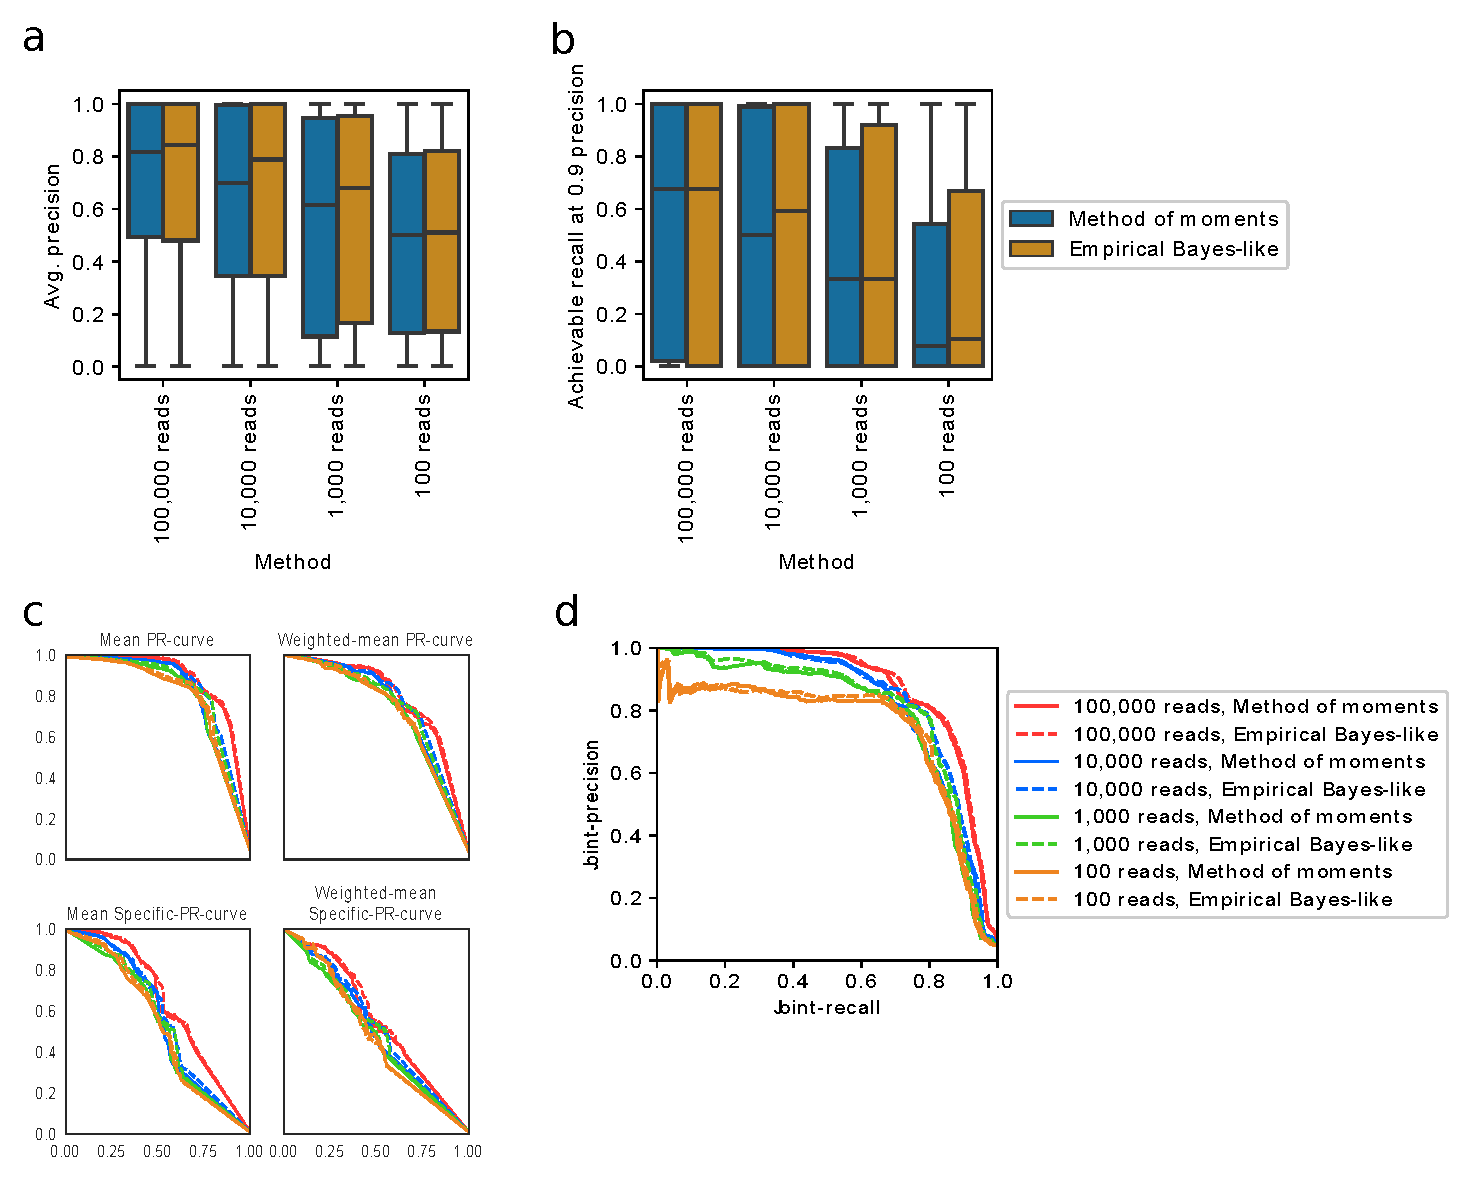
\includegraphics[width=13cm]{figures/empirical_bayes_results.pdf}}
    \caption{\textbf{Results applying empirical Bayes-like estimation approach.}  (a) Comparison between the distributions of average-precision generated by each method across all cell types.  (b) Comparison of the distributions over the highest achievable recalls when precision is fixed at 0.9 across all cell types. (c) Variants of the mean precision-recall curves for comparing the average performance of each method across all samples. (d) The joint-precision recall curves for all methods generating by ranking all sample-cell type output probabilities jointly.}
        \label{fig:shrinkage}
      \end{figure}
 